\documentclass[xcolor=dvipsnames]{beamer} 
\usepackage{verbatim}
\usepackage[utf8]{inputenc}

\usetheme{CambridgeUS} 
\usecolortheme{dolphin}
\setbeamertemplate{items}[ball] 
\setbeamertemplate{blocks}[rounded][shadow=true] 
\newcommand{\spara}[1]{\smallskip\noindent{\bf #1}}
\newcommand{\mpara}[1]{\medskip\noindent{\bf #1}}
\newcommand{\para}[1]{\noindent{\bf #1}}

\newcommand{\bigO}{{\ensuremath{\cal O}}}
\newcommand{\noargsim}{sim}
\newcommand{\wsim}[2]{\noargsim(#1,#2)}
\newcommand{\contextSim}[2]{\mathrm{ContextSim(#1,#2)}}
\newcommand{\textSim}[2]{\mathrm{TextSim(#1,#2)}}
\newcommand{\inLinks}[2]{\mathrm{inLinks(#1,#2)}}
\newcommand{\outLinks}[2]{\mathrm{outLinks(#1,#2)}}
\newcommand{\category}[2]{\mathrm{Category(#1,#2)}}
\newcommand{\textfunc}[2]{Func(#1,#2)}
\newcommand{\wikiJack}[3]{Wk_{#1}(#2,#3)}
\newcommand{\setProximity}[3]{Prox_{#1}(#2,#3)}
\newcommand{\cst}[1]{const_#1}

\newcommand{\ignore}[1]{}

\defbeamertemplate*{footline}{my infolines theme}
{
  \leavevmode%
  \hbox{%
  \begin{beamercolorbox}[wd=.333333\paperwidth,ht=2.25ex,dp=1ex,center]{author in head/foot}%
    \usebeamerfont{author in head/foot}\insertshortauthor~~\insertshortinstitute
  \end{beamercolorbox}%
  \begin{beamercolorbox}[wd=.333333\paperwidth,ht=2.25ex,dp=1ex,center]{title in head/foot}%
    \usebeamerfont{title in head/foot}\insertshorttitle
  \end{beamercolorbox}%
  \begin{beamercolorbox}[wd=.333333\paperwidth,ht=2.25ex,dp=1ex,right]{date in head/foot}%
    \usebeamerfont{date in head/foot}\insertshortdate{}\hspace*{2em}
    \insertframenumber{} / \inserttotalframenumber\hspace*{2ex} 
  \end{beamercolorbox}}%
  \vskip0pt%
}
\title[Challenge 4]{Similarities in Wikipedia }
\author[Oana, Raphaël]{Oana Balalau\inst{1}, Raphaël Bonaque\inst{2}}
\institute[]{
\inst{1}
Télécom ParisTech University
\inst{2}
Inria Saclay \^Ile-de-France
}
\date[EDBT 2015]{EDBT Summer School 2015}


\begin{document}


\begin{frame}

\maketitle
\end{frame}





\section{Challenge}

\begin{frame}{Wikipedia}
 
\begin{center}
\includegraphics[width=0.25\textwidth, height=0.4\paperheight]{media/wikilogo.eps}
\end{center}

Wikipedia is widely used as a source of information. 

Users start from an article and often want more related information.

\end{frame}

\begin{frame}{Finding related information}

Users can obtain more information via links on the page. However:

\begin{itemize}
\item links to similar articles might be missing
\item evaluating existing links relevance is hard
\end{itemize}


\includegraphics[width=0.5\textwidth, height=0.2\paperheight]{media/challenge.eps}

\hspace{-50mm}
\begin{itemize}
\item Compute similarity between articles.
\item Infer new links between articles.
\end{itemize}

\end{frame}



\section{Our approach}


\begin{frame}{When are two pages similar?}

\begin{tabular}{c c}
\hspace{-2mm}\begin{minipage}{.28\textwidth}

\begin{block}{Sources of similarity}

\begin{itemize}
\item Text

\smallskip

\item Context
\begin{itemize}
\item Inlinks
\item Outlinks
\item Categories
\end{itemize}
\end{itemize}

\end{block}
\vspace{1cm}
\begin{tabular}{c | c}
extended & including\\
\hline
intersect & different\\
\end{tabular}

\end{minipage}

&

\begin{minipage}{.6\textwidth}
\begin{tabular}{c | c}

\includegraphics[scale=0.75]{media/c0.eps} & 
\includegraphics[scale=0.75]{media/c1.eps}\\
\hline

\includegraphics[scale=0.75]{media/c2.eps} & 
\includegraphics[scale=0.75]{media/c3.eps}\\
\end{tabular}
\end{minipage}
%Pages discussing related events/topics/concepts use a common set of words.

%\bigskip

%We can find the same words used in similar pages, but sometimes we find synonyms.  


\end{tabular}

\end{frame}


%\begin{frame}{Intuition: Context}


%Related pages link to common pages.
%\bigskip 

%Related pages are linked by common pages.
%\bigskip

%Wikipedia uses categories for grouping together related pages


%\end{frame}

\begin{frame}
We extend the Jaccard similarity coefficient to account for the specifics of Wikipedia:
\begin{align*}	
\wikiJack{f}{S_1}{S_2} =&\ \frac{min(\setProximity{f}{S_1}{S_2}, \setProximity{f}{S_2}{S_1})}{min(|S_1|,|S_2|)}\\
\\
\setProximity{f}{S_1}{S_2} =&\ \sum\limits_{a \in S_1} \max\limits_{b \in S_2}(f(a,b))\\
\end{align*}

Observe that this new coefficient preserves the similarity between two sets if one or both are extended with similar content and that $ 0 \leq \wikiJack{f}{S_1}{S_2} \leq 1 $.

\begin{block}{The original Jaccard similarity}
$$J(S_1,S_2) = \frac{\sum\limits_{a \in S_1} \max\limits_{b \in S_2}(\delta(a,b))}{|S_1 \cup S_1|}$$
\end{block}
\end{frame}


\begin{frame}

We apply this measure on all our sources of similarity: 

\begin{align*}
	\inLinks{a_1}{a_2} =&\ \wikiJack{isSamePage}{inLinks(a_1)}{inLinks(a_2)}\\
	\\
	\outLinks{a_1}{a_2} =&\ \wikiJack{isSamePage}{outLinks(a_1)}{outLinks(a_2)}\\
	\\
	\category{a_1}{a_2} =&\  \wikiJack{intersects}{superCat_3(a_1)}{superCat_3(a_2)}\\
	\\
	\textSim{a_1}{a_2} =&\  \wikiJack{isSynonym}{Stemmed(a_1)}{Stemmed(a_2)}\\
\end{align*}
\end{frame}


\begin{frame}{Sources of similarity}{Categories}


What is the similarity between articles $a_1$ and $a_2$  if we take into account the categories they belong to and the relations between categories?


\begin{center}

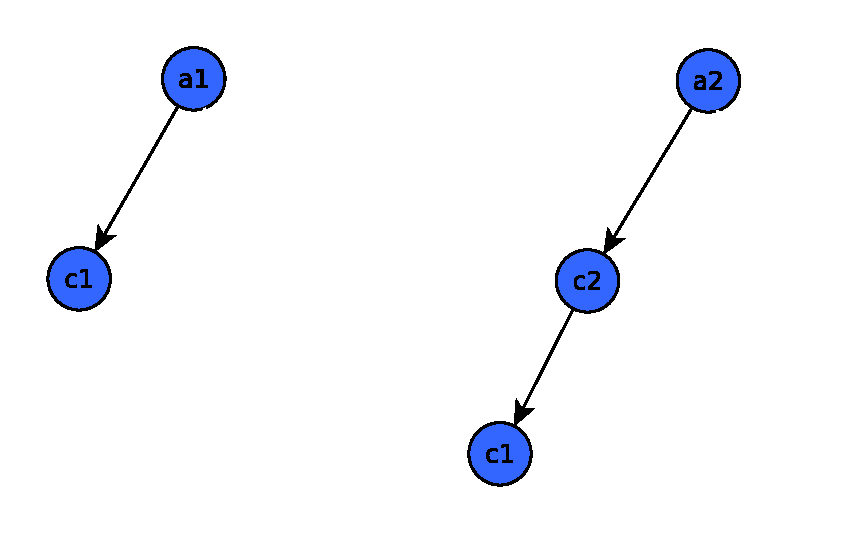
\includegraphics[width=0.6\textwidth, height=0.4\paperheight]{media/sim1.eps}

\end{center}

\end{frame}


\begin{frame}{Sources of similarity}{Categories}

What is the similarity between articles $a_1$ and $a_2$  if we take into account the categories they belong to and the relations between categories?

\begin{center}

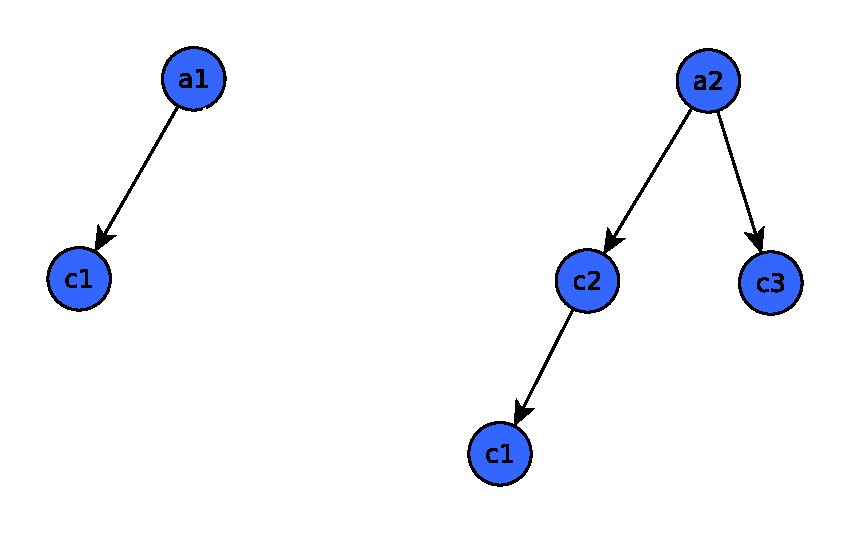
\includegraphics[width=0.6\textwidth, height=0.4\paperheight]{media/sim1.1.eps}

\end{center}

\end{frame}


\begin{frame}{Sources of similarity}{Categories}


What is the similarity between articles $a_1$ and $a_2$  if we take into account the categories they belong to and the relations between categories?


\begin{center}

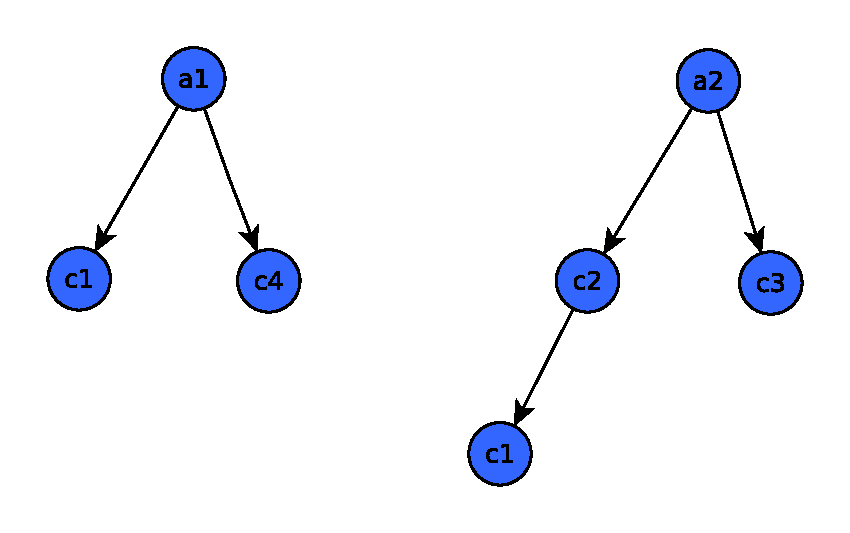
\includegraphics[width=0.6\textwidth, height=0.4\paperheight]{media/sim0.5.eps}

\end{center}

\end{frame}

\begin{frame}{Wikipedia similarity}

By aggregating the similarity components, we get the Wikipedia coefficient of similarity $\wsim$:

\begin{align*}
	\wsim{a_1}{a_2} =&\ &\cst{0} \times \contextSim{a_1}{a_2} \\
	& + &(1 - \cst{0}) \times \textSim{a_1}{a_2} \\
	\\
	\contextSim{a_1}{a_2} =&\ &\cst{1} \times \inLinks{a_1}{a_2}\\
	 	& + &\cst{2} \times \outLinks{a_1}{a_2}\\
	 	& + &(1 - \cst{1} - \cst{2}) \times \category{a_1}{a_2}\\
\end{align*}

where $a_1$ and $a_2$ are two Wikipedia articles. The constants need to be fine tuned by experimental evaluation. 

\end{frame}


\section{Results}
\begin{frame}{Implementation}


\includegraphics[scale=0.3]{media/python-logo.eps}

\bigskip



\includegraphics[scale=0.2]{media/postgres-logo.eps}

\bigskip

The code is available at \url{https://github.com/nyxpho/challenge4EDBT}

\end{frame}

\begin{frame}{Results}

We took pairs of random pages and computed their similarity. 

We obtained for example: 

\begin{center}
\begin{minipage}{\textwidth}
\begin{tabular}{c  c c}

\includegraphics[scale=0.4]{media/moth2.eps} 
& 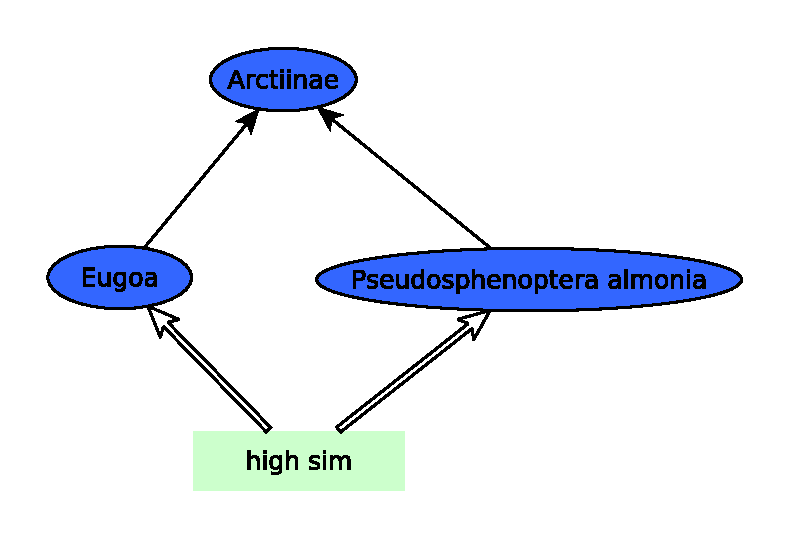
\includegraphics[width=0.6\textwidth, height=0.4\paperheight]{media/moths.eps}
& 
\includegraphics[scale=0.4]{media/moth1.eps}\\

\end{tabular}
\end{minipage}
\end{center}

\end{frame}


\end{document}
